\chapter[Computer-based Mechanisms and Procedures to Gamify CL Sessions]{Computer-based Mechanisms and Procedures to Gamify Collaborative Learning Sessions}
\label{chapter:computer-based-mechanisms-procedures} 

The purpose of this chapter is to show how the ontology OntoGaCLeS, and the GIMF model, presented in previous chapters, can be used in intelligent theory-aware systems to gamify CL sessions, and thus, to deal with the motivation problem caused by the scripted collaboration. 
The \autoref{sec:conceptual-flow-gamify-cl-sessions} presents a conceptual flow to gamify CL sessions proposed as a computer-based procedure that should be used by intelligent theory-aware systems to extract knowledge encoded in the ontology OntoGaCLeS, and then to provide suggestions based on theoretical justification. 
In \autoref{sec:reference-architecture}, a reference architecture based on the conceptual flow to gamify CL sessions is presented. This architecture has been proposed to support the building of computer-based mechanisms that provide support in intelligent-theory aware systems for dealing with the motivation problem caused by the scripted collaboration.

Part of the work described in this chapter was published by the author of this PhD thesis dissertation in the scientific articles:

\begin{itemize}
\item
\aspas{\emph{An Ontology Engineering Approach to Gamify Collaborative Learning Scenarios}} published in the 20\textsuperscript{th} International Conference on Collaboration and Technology, CRIWG 2014, held in Santiago, Chile \cite{ChallcoMoreiraMizoguchiIsotani2014}.

\item
\aspas{\emph{Gamification of Collaborative Learning Scenarios: Structuring Persuasive Strategies Using Game Elements and Ontologies}} published in the 1\textsuperscript{st} International Workshop on Social Computing in Digital Education, SocialEdu 2015, held in Stanford, CA, USA \cite{ChallcoMizoguchiBittencourtIsotani2015}.
\end{itemize}

%%%%%%%%%%%%%%%%%%%%%%%%%%%%%%%%%%
\section[Conceptual Flow to Gamify CL Sessions Using the Ontology OntoGaCLeS]{Conceptual Flow to Gamify Collaborative Learning Sessions Using the Ontology OntoGaCLeS}
\label{sec:conceptual-flow-gamify-cl-sessions}


To avoid the motivation problem caused by the scripted collaboration by means of the gamification, as was mentioned before (in \autoref{chapter:general-background}), it is necessary to solve the context-dependency related to the participants' individual characteristics and traits, and the context-dependency related to the non-game context and target behaviors being gamified. Thus, the gamification should be applied in CL sessions that are the most concrete level of CL scenarios in which the content-domain and participants are well defined, with clear and well-establish group members, CL roles and sequencing of actions to be performed by the group members. 

\autoref{fig:conceptual-flow-gamify-cl-sessions} shows the conceptual flow proposed to gamify CL sessions using the ontology OntoGaCLeS. This flow has been developed from the viewpoint of an instructional designer who employs suggestions given by intelligent-theory aware systems, which in turn use the knowledge encoded in the ontology OntoGaCLeS as a source of information to provide these suggestions.

\begin{figure}[htb]
 \caption{Conceptual flow to gamify collaborative learning sessions using the ontology OntoGaCLeS}
 \label{fig:conceptual-flow-gamify-cl-sessions}
 \centering
 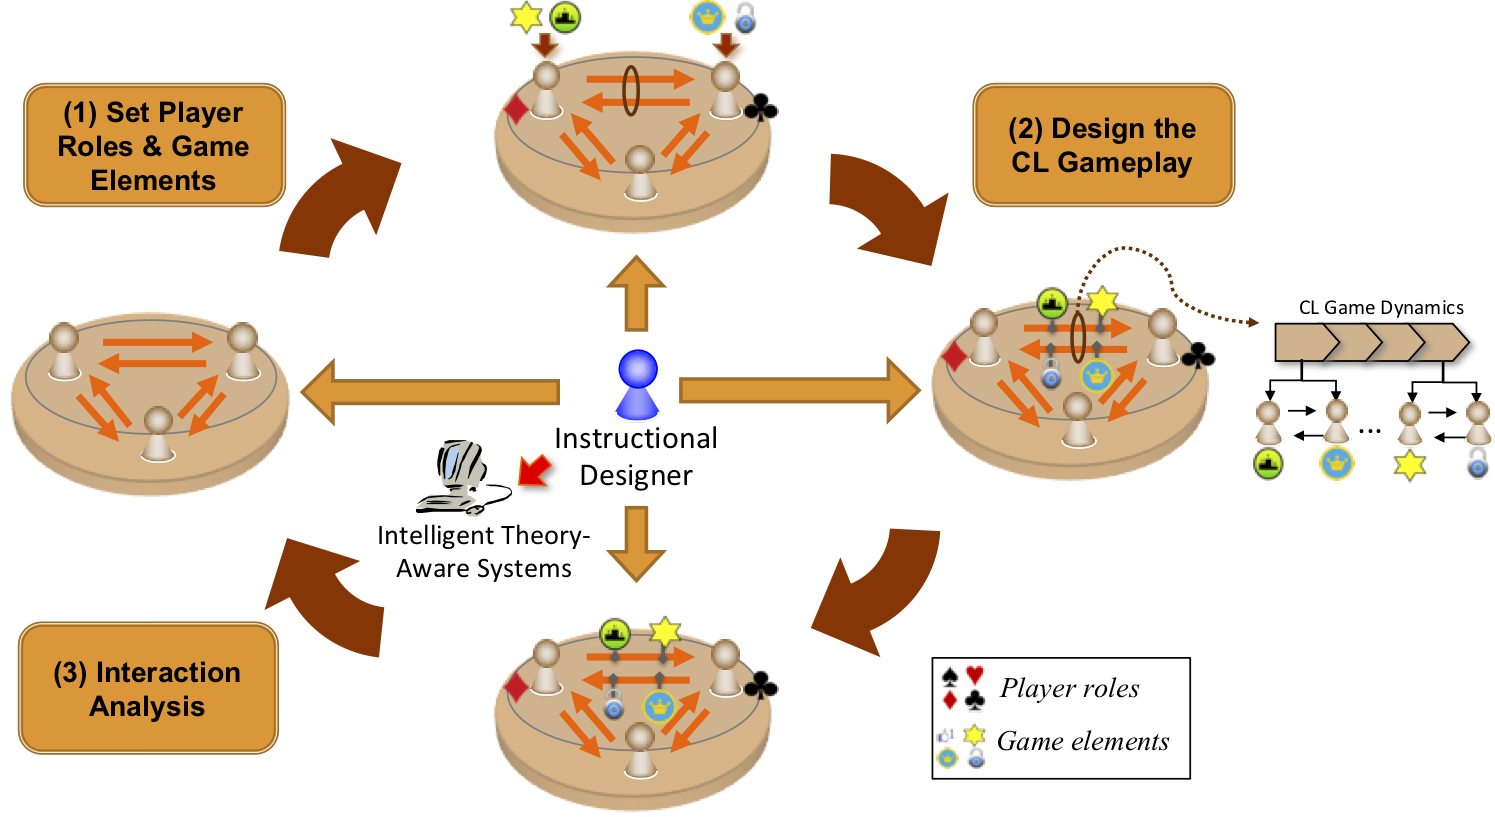
\includegraphics[width=1\textwidth]{images/chap-mechanisms-procedures/conceptual-flow-gamify-cl-sessions.png}
 \fautor
\end{figure}

The basic steps that should be accomplished in the conceptual flow to gamify CL sessions by intelligent-theory aware systems are:

\begin{description}
\item[Step (1):] to set \emph{player roles} and \emph{game elements} for each participant in the CL session,
\item[Step (2):] to design the \emph{CL gameplay} for the CL session, and
\item[Step (3):] to perform an \emph{interaction analysis} over the obtained gamified CL sessions.
\end{description}

\subsection{Step (1): Set Player Roles \& Game Elements}

For each participant in the CL session, an intelligent theory-aware system that uses the ontology OntoGaCLeS to gamify CL sessions should set the player roles and game elements to solve the context-dependency of gamification related to the participants' individual characteristics and traits. The information of player roles and game elements is extracted from ontology-based models to personalize gamification in CL scenarios based on player types models, so that ontological structures to represent gamified CL scenarios (\autoref{subsec:gamified-cl-scenario}) are used to give suggestions in the identification of player roles and game elements that can be assigned for the participants of a CL session.

\begin{algoritmo}
\caption{Algorithm to set player roles and game elements for the participants of a CL session}
\label{algorithm:set-player-roles-game-elements}
\begin{algorithmic}[1]\small
\Procedure{Setup\_Player\_Roles\_and\_Game\_Elements}{CL\_session, Ont\_model}
  \State $set\_gamified\_CL\_scenarios$ $\gets$ \{ \}
  \ForAll{$learner$ in CL\_session}
    \ForAll{$Gamified\_CL\_Scenario$ in Ont\_model}
      \ForAll{$Motivational\_ strategy$ in $Gamified\_CL\_Scenario$}
        \If{is.odd($m$) and ($learner$. $=$ $Motivational\_ strategy$.\emph{I-mot goal (I)})}
          \State add($set\_gamified\_CL\_scenarios$, $Gamified\_CL\_Scenario$)
        \EndIf
      \EndFor
    \EndFor
  \EndFor
\EndProcedure
\end{algorithmic}
\end{algoritmo}

\autoref{algorithm:set-player-roles-game-elements} is described in a narrative form as follows:

\begin{enumerate}
\item
Selecting a subset of ontological structures to represent gamified CL scenarios from an ontology-based model to personalize gamification in CL scenarios based on player types models (Ont\_model). This subset corresponds to ontological structures that would lead the participants to internalize the motivation and satisfy their current motivational needs. This step is accomplished by looking the individual motivational goal (\emph{I-mot goal}) in the individual motivational strategies of (\emph{Y<=I-mot goal}) ontological structures to represent gamified CL scenarios.
\item 
Checking the necessary conditions to play a player role, and setting the priority using the desired conditions


\item 
\end{enumerate}


%to set \emph{player roles} and \emph{game elements} 


%CL scenarios to persuade the participants to follow the interactions defined by the sequencing mechanism of a CSCL script, computer-based mechanisms can be built to help the design of CL gameplay in gamified CL scenarios.


%The building of these structures to define an ontological model comprises the following steps: (1) to identify the player roles that can be assigned for the participants of CL scenario when they are playing a CL role, (2) to identify the restriction and elements of motivational strategies for each pair of identified player roles, and (3) to define individual gameplay strategies for the identified pairs of player roles.


\subsection{Step (2): Design the CL Gameplay}

to design the \emph{CL gameplay} for the CL session by setting up the selected game elements in CL game dynamics that persuade the participants to follow the interactions defined by the CSCL script, and


\subsection{Step (3): Interaction Analysis}

to perform an \emph{interaction analysis} over the obtained gamified CL sessions to propose better solutions by meaningful results obtained by this analysis.

%(2) Design the CL Gameplay

%In the step (1), the designer sets the proper player roles and game elements for each student. In the step (2), he de-signs the CL gameplay as a set of CL game dynamics employing the player roles and game elements that were setting in the first phase. Final-ly, in the step (3), the designer makes an interaction analysis over the obtained gamified CL scenarios to propose better solutions by the meaningful result obtained during the run-time of CSCL scripts.
 
%Fig.1. Flow to gamify a CL scenario in an intelligent theory-aware system. In previous works [2, 4, 5], we define ontological structures that allow us to accomplish the step (1) by the building of models that personalize gamification based on the individual differences of students, such as cur-rent motivation stages, psychological needs and individual personality preferences. To accomplish the step (2), the work [3] propose a set of ontological structures to represent the application of PSs in CL scenarios. To establish these structures employing concepts and semantic relations in our ontology, we use the ontology engineering techniques [24], the Hozo Ontology editor [21], and the model of roles proposed by Mizogu-chi, R. et al. [26].


% The ont-gamified CL sessions have been gamified according to the suggestions given by intelligent-theory aware systems, which in turn used the ontology OntoGaCLeS as information source to give these suggestions. 

%%%%%%%%%%%%%%%%%%%%%%%%%%%%%%%%%%
\section[Reference Architecture for Building Intelligent-theory Aware Systems]{Reference Architecture for Building Intelligent-theory Aware Systems that Use the Ontology OntoGaCLeS}
\label{sec:reference-architecture}

%to provide support in the gamification of CL scenarios

%a reference architecture based on this flow to build computer-based mechanisms that provide support in intelligent-theory aware systems for dealing with the motivation problem caused by the scripted collaboration


%reference architecture for semantic-web intelligent theory-aware systems that will employ the ontology OntoGaCLeS





